\documentclass[12pt]{book}
\usepackage[a4paper, total={6in, 8in}]{geometry}
\usepackage{amssymb}
\usepackage{listings}
\usepackage{color}
\usepackage{graphicx}
\usepackage{subfig}
\usepackage{float}
\definecolor{mygrey}{gray}{.96} % Light Grey
\definecolor{BrickRed}{RGB}{120,0,0}


\def\xbf{\mathbf{x}}
\def\zbf{\mathbf{z}}
\def\xibf{\mathbf{\xi}}
\lstset{
	language=C++,              % choose the language of the code ("language=Verilog" is popular as well)
   tabsize=3,							  % sets the size of the tabs in spaces (1 Tab is replaced with 3 spaces)
	basicstyle=\footnotesize,               % the size of the fonts that are used for the code
	numbers=left,                   % where to put the line-numbers
	numberstyle=\footnotesize,              % the size of the fonts that are used for the line-numbers
	stepnumber=1,                   % the step between two line-numbers. If it's 1 each line will be numbered
	numbersep=5pt,                  % how far the line-numbers are from the code
	backgroundcolor=\color{mygrey}, % choose the background color. You must add \usepackage{color}
	showspaces=false,              % show spaces adding particular underscores
	showstringspaces=false,        % underline spaces within strings
	showtabs=false,                % show tabs within strings adding particular underscores
	frame=single,	                 % adds a frame around the code
	tabsize=3,	                    % sets default tabsize to 2 spaces
	captionpos=b,                   % sets the caption-position to bottom
	breaklines=true,                % sets automatic line breaking
	breakatwhitespace=false,        % sets if automatic breaks should only happen at whitespace
	%escapeinside={\%*}{*)},        % if you want to add a comment within your code
	commentstyle=\color{BrickRed}   % sets the comment style
}

\begin{document}
\title{\textbf{Monte Carlo Simulation Lab}}	
\title{\textbf{Assignment-3}}
\author{Sarthak Agarwal\\(140123031)\\Mathematics and Computing\\IIT Guwahati}
\date{February 9th, 2016}

\maketitle

\newpage
\begin{enumerate}
\item[Q 1] Simulate $5000$ sample of exponential with mean $5$. Draw the histogram and the calculate the mean, maximum and minimum
\end{enumerate}
\noindent{Code for C++}

\begin{lstlisting}
#include <iostream>
#include <cmath>
#include <cstdlib>
#include <stdio.h>

using namespace std;

int main(){
	unsigned long int m=pow(2,31)-1;
	int a=16807,x=12131415,k,r,q;
	float u,num,max=0,min=1234,mean=0	;
	for(int i=0;i<5000;i++){
		q=floor(m/a);
		k=floor(x/q);
		r=(int)m%a;
		x=(a*(x%q)-k*r);
		if(x<0)
			x+=m;
		u=(float)x/m;
		num=-5*log(1-u);
		if(num>max)
			max=num;
		if(num<min)
			min=num;
		mean=(mean*i+num)/(i+1);
	}
	cout<<"mean ="<<mean<<" "<<"maximum="<<max<<" minimum="<<min<<endl;
	return 0;
}
\end{lstlisting}
The output of the code is as follows:\\\\
\begin{lstlisting}
mean =5.19439 maximum=57.7706 minimum=0.000515309
\end{lstlisting}
\newpage
The code in R is shown below:\\
\begin{lstlisting}
x=runif(5000); 
x<-log(1-x)*(-5);
print('Maximum:');
print(max(x));
print('Minimum:');
print(min(x));
print('Mean calculated:');
print(mean(x));
hist(x,main="X ~ Exp(1/5)", xlab="X",ylab="Frequency",xlim=c(0,45),ylim=c(0,900),breaks=50,col="red");
\end{lstlisting}
The output of the R is shown below:\\
\begin{lstlisting}
[1] "Maximum:"
[1] 42.48027
[1] "Minimum:"
[1] 0.001001374
[1] "Mean calculated:"
[1] 5.060602
\end{lstlisting}

The histogram is shown below:
\begin{figure}[H]
	\centering
	\subfloat[$X~Exp(1/5)$]{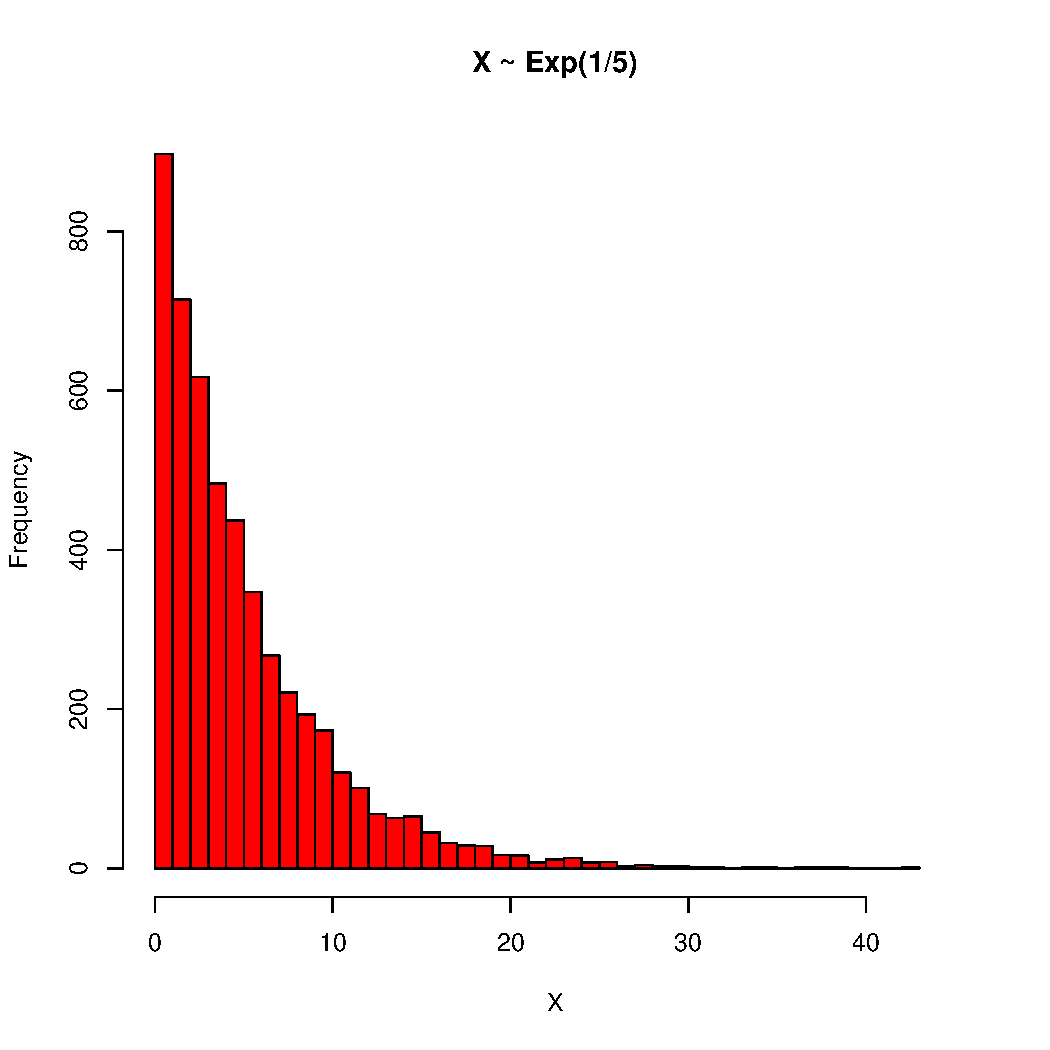
\includegraphics[width=0.6\textwidth]{ass4_1.pdf}}	
\end{figure}
\newpage

\begin{enumerate}
\item[Q 2] Simulate $5000$ sample of Gamma with parameter $n=5$ and $\lambda=5$. Draw the histogram and the calculate the mean, maximum and minimum.
\end{enumerate}
\noindent{Code for C++}

\begin{lstlisting}
#include <iostream>
#include <cmath>
#include <cstdlib>
#include <stdio.h>

using namespace std;

int main(){
	unsigned long int m=pow(2,31)-1;
	int a=16807,x=12131415,k,r,q;
	float u,rand,max=0,min=1234,mean=0,arr[5], temp;
	for(int i=0;i<5;i++)
		arr[i]=0.0;
	for(int i=0;i<5005;i++){
		q=floor(m/a);
		k=floor(x/q);
		r=(int)m%a;
		x=(a*(x%q)-k*r);
		if(x<0)
		{
			x+=m;
		}
		u=float(x)/m;
		arr[i%5]=u;
		if(i>=5){
			temp=(arr[0])*(arr[1])*(arr[2])*(arr[3])*(arr[4]);
			rand=-0.2*log(temp);
			if(rand>max)max=rand;
			if(rand<min)min=rand;
			mean=(mean*i+rand)/(i+1);}
	}
	cout<<"mean ="<<mean<<" "<<"maximum="<<max<<" minimum="<<min<<endl;
	return 0;
}
\end{lstlisting}
The output of the code is as follows:\\\\
\begin{lstlisting}
mean =0.982975 maximum=3.98698 minimum=0.0928889
\end{lstlisting}
\newpage
The code in R is shown below:\\
\begin{lstlisting}
u=runif(5005);
v=NULL;
gamma=NULL;
for(i in 1:5004){
v[(i%%5)+1]<-u[i];
if(i>=5){
temp=(v[1])*(v[2])*(v[3])*(v[5])*(v[4]);
gamma[i-4]=log(temp)*(-0.2);
}
}
print('Maximum:');print(max(gamma));
print('Minimum:');print(min(gamma));
print('Mean calculated:');print(mean(gamma));
hist(gamma,main="X ~ Gamma(5,5)", xlab="X",ylab="Frequency",xlim=c(0,3.5),ylim=c(0,120),breaks=200,col="blue");
\end{lstlisting}
The output of the R is shown below:
\begin{lstlisting}
[1] "Maximum:"
[1] 3.154996
[1] "Minimum:"
[1] 0.06546963
[1] "Mean calculated:"
[1] 0.986534
\end{lstlisting}
\newpage
The histogram is shown below:
\begin{figure}[H]
	\centering
	\subfloat[$X~Gamma(5, 5)$]{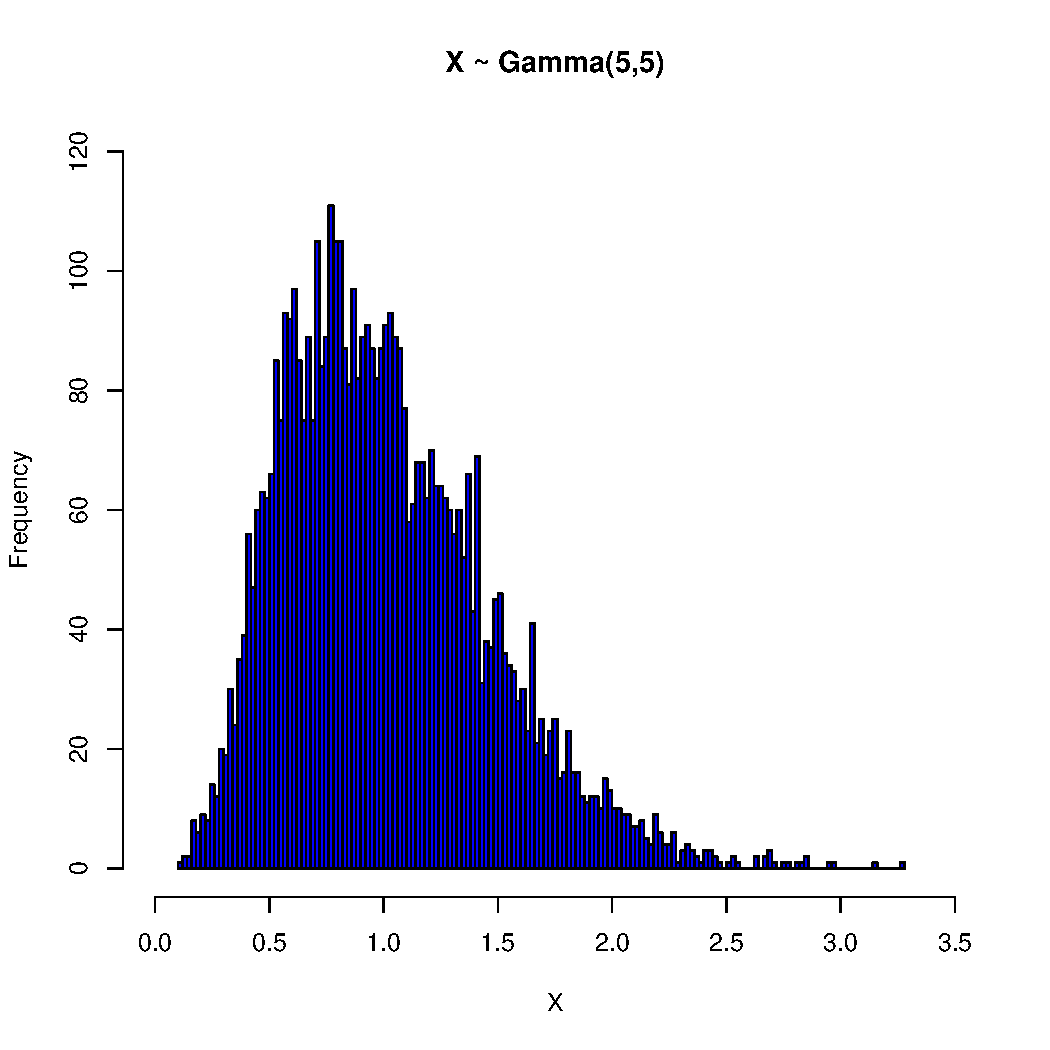
\includegraphics[width=0.6\textwidth]{ass4_2.pdf}}	
\end{figure}
\newpage
\begin{enumerate}
\item[Q 3] Use the rejection method to generate from $$f(x)=20x(1-x)^3, 0<x<1$$
\end{enumerate}
The code in R is shown below:\\
\begin{lstlisting}
f<-function(x)
{
	return (20*x*(1-x)^3);
}
m<-2^13;
a<-189;
b<-56;
x<-4;
y<-2471;
cg<-2;
freq<-array(0,50);
for(i in 1:50000)
{
	x<-(a*x+b)%%m;
	u<-as.double(x)/m;
	y<-(a*y+b+7)%%m;
	v<-as.double(y)/m;
	if(cg*u<=f(v))
		freq[v*50+1]<-freq[v*50+1]+1;
}
barplot(freq, col = "orange");
\end{lstlisting}
\newpage
The histogram formed is as follows:
\begin{figure}[H]
	\centering
	\subfloat[$f(x)=20x(1-x)^3, 0<x<1$]{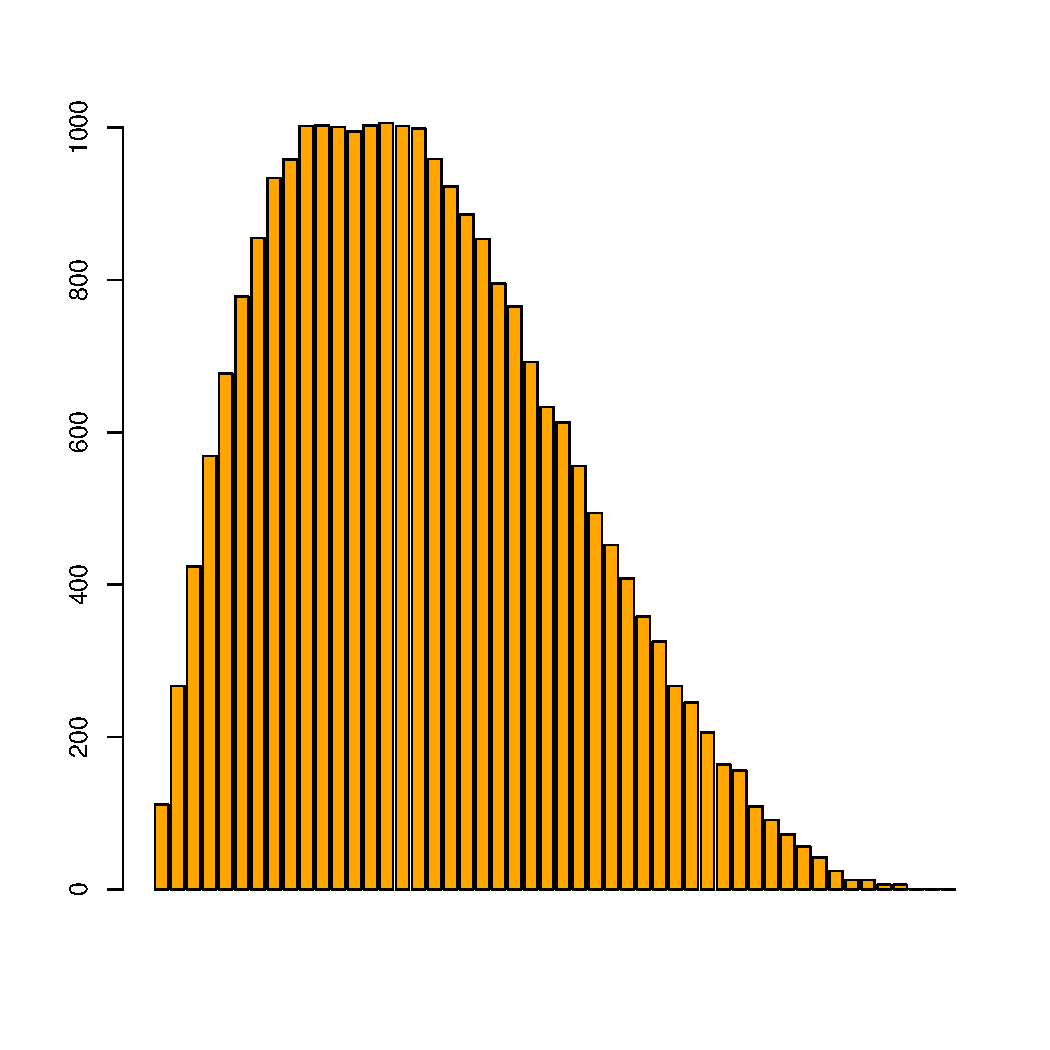
\includegraphics[width=0.6\textwidth]{ass4_3.pdf}}	
\end{figure}
\end{document}